\section{Experiments}
\label{sec:exp}

The experimental section specifies a protocol under which H1--H3 can be falsified and reserves
the table and figure slots that frozen runs will fill. It contains no measured performance.
Every numeric cell is \TODO{PENDING}; a dash means ``not measured or not transcribed'', never
zero. Section~\ref{sec:exp-status} explains which development runs are excluded.

\subsection{Datasets and frozen protocol}
\label{sec:exp-data}

\paragraph{Benchmark.}
We use the public VCSL benchmark~\cite{vcsl2022}. The local frozen copy contains 12,254 ISC
feature files (float32, $[T,256]$, about 4.09~GiB), 97,033 training pairs, 41,798 validation
pairs and 54,630 test pairs; feature lengths range from 3 to 12,590 rows (median 190). The
validation split has 41,798 positive pairs and \emph{no} negatives; the test split has 27,315
positives and 27,315 pairs without a ground-truth key, treated as true negatives by the frozen
local protocol. Both conventions are properties of this release, recorded with SHA-256 hashes
so a later run cannot substitute a different one. GT intervals are boxes on the two
feature-index axes, not dense frame correspondences.

\paragraph{Coordinates and anomalies.}
Predictions are half-open feature-index intervals, never seconds. The audit found a few
degenerate or out-of-range GT intervals (60 out-of-range in 59 validation pairs, maximum excess
108 indices; 4 zero-length/reversed). We keep the original GT, count these cases separately,
and never use GT to correct a prediction or a candidate. A cleaned-subset analysis would be a
separately frozen protocol.

\paragraph{Leakage and threshold discipline.}
The structural configuration is chosen on development data. Each method's own confidence
threshold is then selected on validation and frozen; scores are not calibrated across methods,
so a shared numerical threshold would be unfair. After freezing, test is evaluated exactly
once. No method may drop failed pairs: \textsc{error}/\textsc{skipped} are counted and the
completion rate is reported.

\subsection{Evaluation metric and the four denominators}
\label{sec:exp-metric}

For one pair, let the predictions be $P_1,\dots,P_K$ and the GT boxes $G_1,\dots,G_L$, each a
product of an $A$-interval and a $B$-interval. Let
$O^A_k=\bigcup_{l:P_k\cap G_l\ne\emptyset}(P_k\cap G_l)_A$ be the union of its non-empty
intersections along the query axis, and $O^B_k$ the analogous union along the reference axis.
The official per-pair scores are products of two coverage ratios:
\begin{equation}
\begin{aligned}
P_p&=\frac{\sum_{k}\ell(O^A_k)}{\sum_{k}\ell(P_{k,A})}\cdot
     \frac{\sum_{k}\ell(O^B_k)}{\sum_{k}\ell(P_{k,B})},\\
R_p&=\frac{\sum_{l}\ell(Q^A_l)}{\sum_{l}\ell(G_{l,A})}\cdot
     \frac{\sum_{l}\ell(Q^B_l)}{\sum_{l}\ell(G_{l,B})},
\end{aligned}
\label{eq:metric}
\end{equation}
with $\ell(\cdot)$ interval length and $Q^A_l,Q^B_l$ symmetric over GT boxes; a small
$\epsilon$ guards the denominators. The product, not a minimum or an area IoU, is the official
aggregation. The minimum of two axis IoUs is used only for de-duplicating our predictions
(Section~\ref{sec:method-segments}), and the two must not be confused.

Let $\mathcal{P}$ and $\mathcal{R}$ be the pairs whose per-pair precision and recall are not
exactly 1. The reported scores are
\begin{equation}
\bar P=\frac{1}{|\mathcal{P}|}\sum_{p\in\mathcal{P}}P_p,\qquad
\bar R=\frac{1}{|\mathcal{R}|}\sum_{p\in\mathcal{R}}R_p,\qquad
\mathrm{F1}=\frac{2\bar P\bar R}{\bar P+\bar R},
\label{eq:macro}
\end{equation}
following the official evaluator's sentinel exclusion: empty prediction/empty GT pairs are
dropped, a missing prediction gives $R_p=0$ while its sentinel $P_p=1$ is dropped, and a
false alarm on a negative gives $P_p=0$ while the sentinel $R_p=1$ is dropped. Two consequences
matter. First, a correctly rejected negative contributes to neither mean, so its success is
invisible and a separate negative FAR is necessary. Second, exclusion is by value, not cause:
a genuine perfect prediction also has $P_p=1$ and is dropped. We preserve this for
comparability and report how many pairs were excluded.

\paragraph{Four denominators.}
Every run reports: \texttt{n\_expected} (list size), \texttt{n\_processed}
(\textsc{ok}+\textsc{empty}), \texttt{n\_precision\_denom}=$|\mathcal{P}|$, and
\texttt{n\_recall\_denom}=$|\mathcal{R}|$. The last two are the true macro denominators, not
simply ``non-empty predictions'' and ``positive pairs''. We also report
\texttt{n\_pairs\_with\_gt}, \texttt{n\_pairs\_with\_pred},
\texttt{excluded\_precision\_eq\_1} and \texttt{excluded\_recall\_eq\_1}.

\paragraph{Negative-pair FAR.}
On test, the negative-pair false alarm rate is the fraction of the 27,315 true negatives for
which the frozen system outputs at least one segment. It is not reported on validation, which
has no negatives; that cell reads \texttt{N/A (positive-only split)}.

\paragraph{Diagnostic metrics.}
For H1/H2 we also define candidate recall (fraction of GT segments matched by a candidate at
$\minIoU\ge\theta$), boundary MAE (mean absolute endpoint error in frames over matched
segments), negative FAR, and tube cells evaluated ($\sum_rL_rW_r$ over attempted passes). These
are labelled custom diagnostics. VCSL provides interval boxes, not dense correspondence, so we
do not claim a frame-level correspondence recall.

\subsection{Baselines and the Simple Sparse-to-Band gate}
\label{sec:exp-baselines}

HV~\cite{douze2016,jiang2014}, TN~\cite{tan2009}, DP and DTW~\cite{chou2015,smith1981} run
under the same features, pair lists, GT and evaluator. They do not train a localizer; that is a
property of the method, not of our run. SPD~\cite{spd2021} detects aligned regions on a
similarity map and is trained; TransVCL~\cite{transvcl2023} enhances features with attention
and regresses boxes with a detection head; RTR~\cite{rtr2024} adds regional tokens and
self-supervised pairs; FiGVCL~\cite{figvcl2025} targets fine-grained transformations. These are
loaded pretrained and \emph{not} retrained here, so the ``trained in this work'' column is No
everywhere without implying that the method is training-free. Methods whose features or
protocol cannot be aligned with the frozen pipeline are reported as quoted reference values in
a separate block and excluded from ranking.

\paragraph{TransVCL chunking.}
TransVCL splits features into chunks of at most 1,200 frames, enumerates chunk pairs, and
shifts predictions back by the chunk offsets~\cite{transvcl2023}. It therefore does not
allocate the full $M\times N$ matrix for a long pair. Its per-video-pair latency must be
obtained by summing chunk-pair times, not by quoting one chunk.

\paragraph{The gate.}
Because every ingredient is classical, a weak baseline would prove nothing. We define a
strong, simple baseline: one grid at fixed stride $s$ $\rightarrow$ mutual Top-$K$ anchors
above $\tau$ $\rightarrow$ standard RANSAC line fit $\rightarrow$ fixed half-width band
$\rightarrow$ standard zero-floored Smith--Waterman alignment $\rightarrow$ the same threshold
sweep and de-duplication. It has no dual-axis gap splitting, no independent phases, no
multi-path extraction, and no min-IoU-specific logic. FastVCL is compared at the same coarse
dot-product budget and hardware. If it does not beat this baseline on F1, short-segment recall
or boundary MAE, the honest conclusion is \texttt{NOVELTY\_GAP}; E1 makes that outcome
impossible to hide.

\subsection{E0: external comparison}
\label{sec:exp-e0}

E0 compares FastVCL with HV, TN, DP, DTW, TransVCL and, if its features align, SPD, under the
same files, evaluator, machine and timing boundary, with per-method thresholds frozen on
validation. Table~\ref{tab:main} separates quoted values (different features/protocols) from
values measured here; no ranking crosses the separator.

\subsection{E1: simple-baseline gate}
\label{sec:exp-e1}

E1 adds one mechanism at a time to the Simple Sparse-to-Band baseline with the coarse budget,
candidate count and hardware fixed. The headline comparison is the full pipeline against the
full baseline. A mechanism is retained only if it improves F1, short-segment recall or boundary
MAE beyond the seed variance of the stochastic fitting stage. If none survives, the paper must
be reframed around the negative result.

\subsection{E2: sampling and phase (H1)}
\label{sec:exp-e2}

E2 varies only the coarse sampling: stride 4; stride 2; nested $\{2,4,8\}$ with and without
coordinate de-duplication; independent phase pairs; and a single fine grid at the same
\emph{executed} dot-product budget. Each point records $Q^{\mathrm{actual}}_{\mathrm{coarse}}$,
$|\Anch|$, removed cross-grid duplicates, candidate recall and coarse latency, bucketed by GT
length ($<15$, $[15,60)$, $\ge60$ frames). Two controls are mandatory: the iso-budget
single-grid comparison and the de-duplication-off run. Without them a ``multi-scale'' gain
cannot be separated from a budget increase or double-counted support.

\subsection{E3: refinement and restart semantics (H2)}
\label{sec:exp-e3}

E3 locks the candidates and compares four refinements on identical tracks: (a) the coarse
support box; (b) global DTW without a zero floor; (c) unconditional continuation; (d) the
proposed \eqref{eq:localdp}. Differences are then attributable to refinement, not upstream
randomness. We report $\bar P/\bar R/\mathrm{F1}$, boundary MAE on matched segments, the
false-merge rate on the two counterexample regimes of Section~\ref{sec:method-dp}, refinement
latency and tube cells. A GT-induced tube runs only as a labelled oracle diagnostic.

\subsection{E4: single-factor ablations}
\label{sec:exp-e4}

E4 changes one item per row: remove dual-axis support; remove gap splitting; replace min-IoU
with joint-envelope IoU; sweep $e_A$; sweep $w_r$. The seed is fixed per pair and headline rows
repeat over five seeds. We report candidate-track count, $\sum_rL_rW_r$, the spurious-track
fraction under repeated texture, F1 and latency. ``No geometry'' is \emph{not} ``output
nothing'': its replacement proposes local windows around the highest-scoring anchor clusters at
the same dot-product budget.

\subsection{E5: implementation cost and memory (H3)}
\label{sec:exp-e5}

E5 compares three implementations of the same refinement: the prototype predecessor scan, a
direct-offset indexing, and a vectorised full-matrix DP baseline. It reports stage shares
(normalisation, coarse matching, RANSAC, band similarity, DP, traceback, post-processing),
executed dot products, tube cells, peak RSS and, if available, GPU memory. GPU numbers appear
only after a real-hardware parity test; a kernel that never ran on a GPU is not evidence of
speed. The timing boundary is $\Tloc$: from raw features resident in CPU memory and operators
initialised to in-memory five-column predictions. Feature I/O, export, process start-up and
video decoding are separate. Measurements disable per-tile profiling, include a warm-up and at
least three rounds; GPU timing is synchronised at both ends.

\subsection{Results (pending)}
\label{sec:exp-results}

\begin{table*}[t]
\centering
\caption{\textbf{Main comparison under the frozen VCSL protocol.}
Upper block: values quoted from the original papers; features and protocols differ, so these
rows are \emph{not} ranked against the lower block. Lower block: to be measured here with
the same ISC features, pair lists, GT and evaluator, with a per-method threshold selected on
validation and frozen. \textbf{All numeric cells are \TODO{PENDING}}; ``--'' means not
measured or not transcribed, never zero. Validation negative FAR is \texttt{N/A}
(positive-only split); the FAR column is test-only.}
\label{tab:main}
\scriptsize
\setlength{\tabcolsep}{4pt}
\renewcommand{\arraystretch}{1.05}
\begin{tabular}{@{}l c c c c c@{}}
\toprule
Method (venue) & Learned & Val P/R/F1 & Test P/R/F1 & FAR (\%) & $\Tloc$ (ms) \\
\midrule
\multicolumn{6}{@{}l}{\emph{Quoted reference values --- different protocol, not ranked here}}\\
HV (VCSL'22)          & No  & -- & -- & -- & -- \\
TN (VCSL'22)          & No  & -- & -- & -- & -- \\
DP (VCSL'22)          & No  & -- & -- & -- & -- \\
DTW (VCSL'22)         & No  & -- & -- & -- & -- \\
SPD (MM'21)           & Yes & -- & -- & -- & -- \\
TransVCL (AAAI'23)    & Yes & -- & -- & -- & -- \\
RTR (ECCV'24)         & Yes & -- & -- & -- & -- \\
TCSVT'24              & No  & -- & -- & -- & -- \\
FiGVCL (TPAMI'25)     & Yes & -- & -- & -- & -- \\
\midrule
\multicolumn{6}{@{}l}{\emph{Frozen protocol --- same ISC features, pair list, GT and evaluator}}\\
HV                    & No  & -- & -- & -- & -- \\
TN                    & No  & -- & -- & -- & -- \\
DP                    & No  & -- & -- & -- & -- \\
DTW                   & No  & -- & -- & -- & -- \\
TransVCL              & Yes & -- & -- & -- & -- \\
SPD                   & Yes & -- & -- & -- & -- \\
Simple Sparse-to-Band & No  & -- & -- & -- & -- \\
\textbf{FastVCL (proposed)} & No & -- & -- & -- & -- \\
\bottomrule
\end{tabular}
\vspace{3pt}
\par\raggedright\footnotesize
Sources: HV/TN/DP/DTW and the VCSL protocol~\cite{vcsl2022}; SPD~\cite{spd2021};
TransVCL~\cite{transvcl2023}; RTR~\cite{rtr2024}; TCSVT~\cite{tcsvt2024};
FiGVCL~\cite{figvcl2025}. No method is trained in this work. Every frozen-protocol run must
report the four denominators defined in Section~\ref{sec:exp-metric}. Simple Sparse-to-Band
is the novelty gate (Section~\ref{sec:exp-baselines}). TCSVT 2024 uses learned image
descriptors but a non-learned temporal-consistency localizer, so it is marked No.
\end{table*}

\begin{table*}[t]
\centering
\caption{\textbf{System efficiency, memory and stage breakdown.}
Same machine, feature files and protocol; per-tile profiling off; one warm-up and at least
three measured rounds. $\Tloc$ covers normalisation through in-memory prediction and excludes
feature I/O, export and video decoding. TransVCL latency is summed over chunk pairs per video
pair. CPU-only methods report \texttt{N/A} for GPU memory. \TODO{All entries are pending.}}
\label{tab:efficiency}
\scriptsize
\setlength{\tabcolsep}{3pt}
\begin{tabular}{@{}l l c c c c c@{}}
\toprule
Method & HW & Pairs & $\Tloc$ mean/P50/P95 & Thr. & RSS/VRAM & F1 \\
\midrule
HV       & CPU & -- / 41{,}800 & -- / -- / -- & -- & -- / N/A & -- \\
TN       & CPU & -- / 41{,}800 & -- / -- / -- & -- & -- / N/A & -- \\
DP       & CPU & -- / 41{,}800 & -- / -- / -- & -- & -- / N/A & -- \\
DTW      & CPU & -- / 41{,}800 & -- / -- / -- & -- & -- / N/A & -- \\
TransVCL & GPU & -- / 41{,}800 & -- / -- / -- & -- & -- / -- & -- \\
Simple Sparse-to-Band & CPU & -- / 41{,}800 & -- / -- / -- & -- & -- / N/A & -- \\
FastVCL (proposed) & CPU & -- / 41{,}800 & -- / -- / -- & -- & -- / N/A & -- \\
FastVCL (CUDA path) & GPU & -- / 41{,}800 & -- / -- / -- & -- & -- / -- & -- \\
\bottomrule
\end{tabular}
\vspace{3pt}
\par\raggedright\footnotesize
Exact CPU/GPU models, thread counts and precision are pending. ``Pairs done/total'' counts
\textsc{error}/\textsc{skipped} explicitly. The CUDA row exists only after real-hardware
acceptance; until then \TODO{no GPU kernel has executed}.
\end{table*}

\begin{table*}[t]
\centering
\caption{\textbf{Controlled mechanism and hypothesis ablations (H1--H3).}
Each row changes exactly one mechanism or hyperparameter. ``Dots'' is the executed dot-product
count (both Top-$K$ directions and tie passes); ``cells'' is $\sum_r L_rW_r$ over attempted
passes. Candidate recall and boundary MAE are custom diagnostics
(Section~\ref{sec:exp-metric}), not the official metric. \TODO{All entries are pending.}}
\label{tab:ablation}
\scriptsize
\setlength{\tabcolsep}{3pt}
\renewcommand{\arraystretch}{1.02}
\begin{tabular}{@{}l l l c c c c c c@{}}
\toprule
Exp & Variant & Change & Dots & Cells & Cand.R & Bnd.MAE & F1 & Tloc \\
\midrule
E1 & Simple STB & reference & -- & -- & -- & -- & -- & -- \\
E1 & FastVCL & +dual-axis, phases & -- & -- & -- & -- & -- & -- \\
\midrule
E2 & stride 2 & $s=2$ & -- & -- & -- & -- & -- & -- \\
E2 & stride 4 & $s=4$ & -- & -- & -- & -- & -- & -- \\
E2 & multi-scale & add $\{2,8\}$ & -- & -- & -- & -- & -- & -- \\
E2 & no de-dup & drop dedup & -- & -- & -- & -- & -- & -- \\
E2 & indep.\ phases & add offsets & -- & -- & -- & -- & -- & -- \\
\midrule
E3 & coarse support box & no refinement & -- & -- & -- & -- & -- & -- \\
E3 & band DTW & global & -- & -- & -- & -- & -- & -- \\
E3 & continuation & prototype & -- & -- & -- & -- & -- & -- \\
E3 & zero-floored DP & proposed \eqref{eq:localdp} & -- & -- & -- & -- & -- & -- \\
\midrule
E4 & no support & support/span off & -- & -- & -- & -- & -- & -- \\
E4 & no split & one run/line & -- & -- & -- & -- & -- & -- \\
E4 & joint IoU & replace min-IoU & -- & -- & -- & -- & -- & -- \\
E4 & sweep & $e_A$, $w_r$ & -- & -- & -- & -- & -- & -- \\
\midrule
E5 & scan & prototype & -- & -- & -- & -- & -- & -- \\
E5 & offset & $O(LW)$ & -- & -- & -- & -- & -- & -- \\
\bottomrule
\end{tabular}
\vspace{3pt}
\par\raggedright\footnotesize
Rows are grouped by experiment; within E2--E4 only the named factor changes. Multi-scale rows
need an equal-budget single-stride-2 control. RANSAC seed is fixed per pair; headline rows are
repeated over five seeds.
\end{table*}
Tables~\ref{tab:main}--\ref{tab:ablation} are structured and deliberately empty. They will be
filled only from frozen runs whose status files account for every selected pair. No such run
exists: the largest development execution covers 41,797 of 41,798 validation pairs but contains
one unhandled error and uses an unfrozen development configuration, and no test split has been
scored. We therefore report no accuracy, latency, memory or negative-FAR number, and we do not
use those diagnostics as results (Section~\ref{sec:exp-status}).

\subsection{Accuracy--cost plane}
\label{sec:exp-tradeoff}

Figure~\ref{fig:tradeoff} reserves the plane required by H3: measured per-pair $\Tloc$ on the
horizontal axis and VCSL F1 on the vertical axis, with operating points obtained by varying
each method's threshold after its structure is frozen. A method that only moves along the curve
has not improved the trade-off; one that dominates the curve has. The figure contains no curve
and no point in this draft.

\begin{figure}[t]
  \centering
  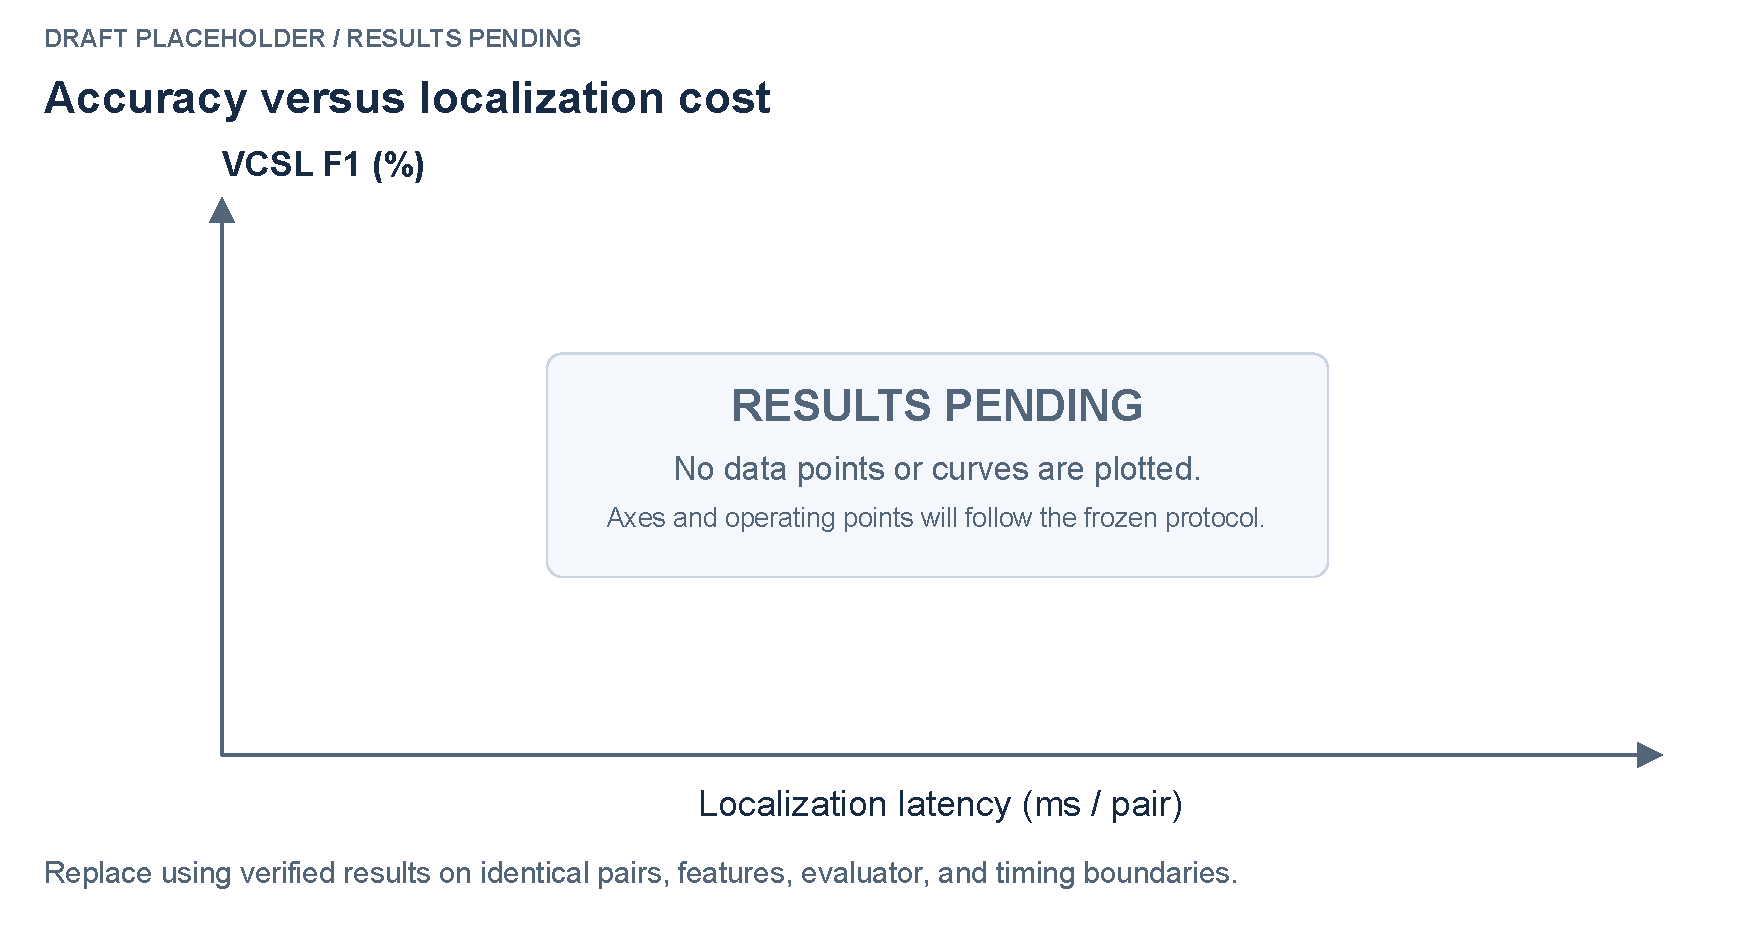
\includegraphics[width=\columnwidth]{figures/fig_4_tradeoff.pdf}
  \caption{\textbf{Reserved accuracy--cost plane (\emph{results pending}).}
  No data points or fitted curves are shown. Axes are fixed so that frozen runs can be plotted
  without changing the layout: VCSL F1 versus measured per-pair localization latency. Points
  will be produced only from verified runs with identical pairs, features, evaluator and timing
  boundary.}
  \label{fig:tradeoff}
\end{figure}

\subsection{Threats to validity and current evidence status}
\label{sec:exp-status}

\paragraph{H1.} A coarse stage that misses many short copies cannot be rescued by
refinement. The sampling bound \eqref{eq:shortbound} defines the structural regime; length-
bucketed candidate recall in E2 is the measurement.

\paragraph{H2.} A refinement that improves endpoints only by widening the search until it
approaches the full matrix does not test the finite-tube hypothesis. E3 fixes the candidates
and reports tube cells so that a gain bought by brute force is visible.

\paragraph{H3.} Python loops, predecessor scans, allocation and transfer overhead can consume
the arithmetic saving. The prototype's predecessor scan is the concrete risk: its per-cell cost
is $O(W_r)$ instead of $O(1)$, turning the ideal $O(L_rW_r)$ into $O(P_rL_rW_r^2)$. E5 measures
both.

\paragraph{What is excluded.} Development executions on 20--1,000 pairs are not results; the
\texttt{dev1000} metrics file is computed over 200 scored pairs, not 1,000, and a directory
name or a \texttt{COMPLETE} label does not change that. The near-complete validation run has
one error and an unfrozen configuration. Synthetic runs are engineering checks. No GPU kernel
has executed on hardware, so no GPU claim is made. Run identifiers and the full audit are in
the supplementary material.
